\documentclass[1p]{elsarticle_modified}
%\bibliographystyle{elsarticle-num}

%\usepackage[colorlinks]{hyperref}
%\usepackage{abbrmath_seonhwa} %\Abb, \Ascr, \Acal ,\Abf, \Afrak
\usepackage{amsfonts}
\usepackage{amssymb}
\usepackage{amsmath}
\usepackage{amsthm}
\usepackage{scalefnt}
\usepackage{amsbsy}
\usepackage{kotex}
\usepackage{caption}
\usepackage{subfig}
\usepackage{color}
\usepackage{graphicx}
\usepackage{xcolor} %% white, black, red, green, blue, cyan, magenta, yellow
\usepackage{float}
\usepackage{setspace}
\usepackage{hyperref}

\usepackage{tikz}
\usetikzlibrary{arrows}

\usepackage{multirow}
\usepackage{array} % fixed length table
\usepackage{hhline}

%%%%%%%%%%%%%%%%%%%%%
\makeatletter
\renewcommand*\env@matrix[1][\arraystretch]{%
	\edef\arraystretch{#1}%
	\hskip -\arraycolsep
	\let\@ifnextchar\new@ifnextchar
	\array{*\c@MaxMatrixCols c}}
\makeatother %https://tex.stackexchange.com/questions/14071/how-can-i-increase-the-line-spacing-in-a-matrix
%%%%%%%%%%%%%%%

\usepackage[normalem]{ulem}

\newcommand{\msout}[1]{\ifmmode\text{\sout{\ensuremath{#1}}}\else\sout{#1}\fi}
%SOURCE: \msout is \stkout macro in https://tex.stackexchange.com/questions/20609/strikeout-in-math-mode

\newcommand{\cancel}[1]{
	\ifmmode
	{\color{red}\msout{#1}}
	\else
	{\color{red}\sout{#1}}
	\fi
}

\newcommand{\add}[1]{
	{\color{blue}\uwave{#1}}
}

\newcommand{\replace}[2]{
	\ifmmode
	{\color{red}\msout{#1}}{\color{blue}\uwave{#2}}
	\else
	{\color{red}\sout{#1}}{\color{blue}\uwave{#2}}
	\fi
}

\newcommand{\Sol}{\mathcal{S}} %segment
\newcommand{\D}{D} %diagram
\newcommand{\A}{\mathcal{A}} %arc


%%%%%%%%%%%%%%%%%%%%%%%%%%%%%5 test

\def\sl{\operatorname{\textup{SL}}(2,\Cbb)}
\def\psl{\operatorname{\textup{PSL}}(2,\Cbb)}
\def\quan{\mkern 1mu \triangleright \mkern 1mu}

\theoremstyle{definition}
\newtheorem{thm}{Theorem}[section]
\newtheorem{prop}[thm]{Proposition}
\newtheorem{lem}[thm]{Lemma}
\newtheorem{ques}[thm]{Question}
\newtheorem{cor}[thm]{Corollary}
\newtheorem{defn}[thm]{Definition}
\newtheorem{exam}[thm]{Example}
\newtheorem{rmk}[thm]{Remark}
\newtheorem{alg}[thm]{Algorithm}

\newcommand{\I}{\sqrt{-1}}
\begin{document}

%\begin{frontmatter}
%
%\title{Boundary parabolic representations of knots up to 8 crossings}
%
%%% Group authors per affiliation:
%\author{Yunhi Cho} 
%\address{Department of Mathematics, University of Seoul, Seoul, Korea}
%\ead{yhcho@uos.ac.kr}
%
%
%\author{Seonhwa Kim} %\fnref{s_kim}}
%\address{Center for Geometry and Physics, Institute for Basic Science, Pohang, 37673, Korea}
%\ead{ryeona17@ibs.re.kr}
%
%\author{Hyuk Kim}
%\address{Department of Mathematical Sciences, Seoul National University, Seoul 08826, Korea}
%\ead{hyukkim@snu.ac.kr}
%
%\author{Seokbeom Yoon}
%\address{Department of Mathematical Sciences, Seoul National University, Seoul, 08826,  Korea}
%\ead{sbyoon15@snu.ac.kr}
%
%\begin{abstract}
%We find all boundary parabolic representation of knots up to 8 crossings.
%
%\end{abstract}
%\begin{keyword}
%    \MSC[2010] 57M25 
%\end{keyword}
%
%\end{frontmatter}

%\linenumbers
%\tableofcontents
%
\newcommand\colored[1]{\textcolor{white}{\rule[-0.35ex]{0.8em}{1.4ex}}\kern-0.8em\color{red} #1}%
%\newcommand\colored[1]{\textcolor{white}{ #1}\kern-2.17ex	\textcolor{white}{ #1}\kern-1.81ex	\textcolor{white}{ #1}\kern-2.15ex\color{red}#1	}

{\Large $\underline{11a_{76}~(K11a_{76})}$}

\setlength{\tabcolsep}{10pt}
\renewcommand{\arraystretch}{1.6}
\vspace{1cm}\begin{tabular}{m{100pt}>{\centering\arraybackslash}m{274pt}}
\multirow{5}{120pt}{
	\centering
	\includegraphics[width=112pt]{../../../GIT/diagram.site/Diagrams/png/325_11a_76.png}\\
\ \ \ A knot diagram\footnotemark}&
\allowdisplaybreaks
\textbf{Linearized knot diagam} \\
\cline{2-2}
 &
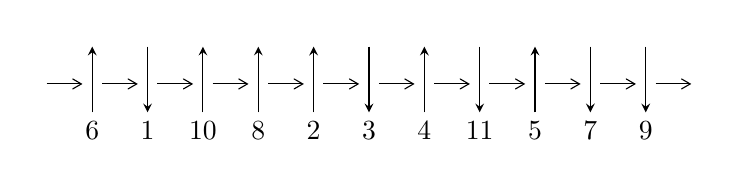
\begin{tikzpicture}[x=20pt, y=17pt]
	% nodes
	\node (C0) at (0, 0) {};
	\node (C1) at (1, 0) {};
	\node (C1U) at (1, +1) {};
	\node (C1D) at (1, -1) {6};

	\node (C2) at (2, 0) {};
	\node (C2U) at (2, +1) {};
	\node (C2D) at (2, -1) {1};

	\node (C3) at (3, 0) {};
	\node (C3U) at (3, +1) {};
	\node (C3D) at (3, -1) {10};

	\node (C4) at (4, 0) {};
	\node (C4U) at (4, +1) {};
	\node (C4D) at (4, -1) {8};

	\node (C5) at (5, 0) {};
	\node (C5U) at (5, +1) {};
	\node (C5D) at (5, -1) {2};

	\node (C6) at (6, 0) {};
	\node (C6U) at (6, +1) {};
	\node (C6D) at (6, -1) {3};

	\node (C7) at (7, 0) {};
	\node (C7U) at (7, +1) {};
	\node (C7D) at (7, -1) {4};

	\node (C8) at (8, 0) {};
	\node (C8U) at (8, +1) {};
	\node (C8D) at (8, -1) {11};

	\node (C9) at (9, 0) {};
	\node (C9U) at (9, +1) {};
	\node (C9D) at (9, -1) {5};

	\node (C10) at (10, 0) {};
	\node (C10U) at (10, +1) {};
	\node (C10D) at (10, -1) {7};

	\node (C11) at (11, 0) {};
	\node (C11U) at (11, +1) {};
	\node (C11D) at (11, -1) {9};
	\node (C12) at (12, 0) {};

	% arrows
	\draw[->,>={angle 60}]
	(C0) edge (C1) (C1) edge (C2) (C2) edge (C3) (C3) edge (C4) (C4) edge (C5) (C5) edge (C6) (C6) edge (C7) (C7) edge (C8) (C8) edge (C9) (C9) edge (C10) (C10) edge (C11) (C11) edge (C12) ;	\draw[->,>=stealth]
	(C1D) edge (C1U) (C2U) edge (C2D) (C3D) edge (C3U) (C4D) edge (C4U) (C5D) edge (C5U) (C6U) edge (C6D) (C7D) edge (C7U) (C8U) edge (C8D) (C9D) edge (C9U) (C10U) edge (C10D) (C11U) edge (C11D) ;
	\end{tikzpicture} \\
\hhline{~~} \\& 
\textbf{Solving Sequence} \\ \cline{2-2} 
 &
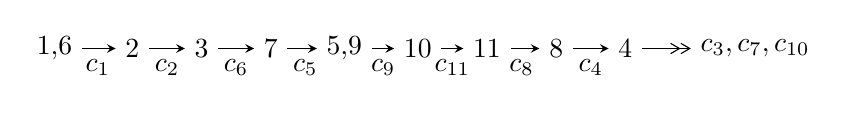
\begin{tikzpicture}[x=25pt, y=7pt]
	% node
	\node (A0) at (-1/8, 0) {1,6};
	\node (A1) at (1, 0) {2};
	\node (A2) at (2, 0) {3};
	\node (A3) at (3, 0) {7};
	\node (A4) at (65/16, 0) {5,9};
	\node (A5) at (41/8, 0) {10};
	\node (A6) at (49/8, 0) {11};
	\node (A7) at (57/8, 0) {8};
	\node (A8) at (65/8, 0) {4};
	\node (C1) at (1/2, -1) {$c_{1}$};
	\node (C2) at (3/2, -1) {$c_{2}$};
	\node (C3) at (5/2, -1) {$c_{6}$};
	\node (C4) at (7/2, -1) {$c_{5}$};
	\node (C5) at (37/8, -1) {$c_{9}$};
	\node (C6) at (45/8, -1) {$c_{11}$};
	\node (C7) at (53/8, -1) {$c_{8}$};
	\node (C8) at (61/8, -1) {$c_{4}$};
	\node (A9) at (10, 0) {$c_{3},c_{7},c_{10}$};

	% edge
	\draw[->,>=stealth]	
	(A0) edge (A1) (A1) edge (A2) (A2) edge (A3) (A3) edge (A4) (A4) edge (A5) (A5) edge (A6) (A6) edge (A7) (A7) edge (A8) ;
	\draw[->>,>={angle 60}]	
	(A8) edge (A9);
\end{tikzpicture} \\ 

\end{tabular} \\

\footnotetext{
The image of knot diagram is generated by the software ``\textbf{Draw programme}" developed by Andrew Bartholomew(\url{http://www.layer8.co.uk/maths/draw/index.htm\#Running-draw}), where we modified some parts for our purpose(\url{https://github.com/CATsTAILs/LinksPainter}).
}\phantom \\ \newline 
\centering \textbf{Ideals for irreducible components\footnotemark of $X_{\text{par}}$} 
 
\begin{align*}
I^u_{1}&=\langle 
-3.57893\times10^{38} u^{71}-8.42472\times10^{38} u^{70}+\cdots+5.29862\times10^{37} b-4.92590\times10^{38},\\
\phantom{I^u_{1}}&\phantom{= \langle  }-2.62436\times10^{38} u^{71}-6.46971\times10^{38} u^{70}+\cdots+5.29862\times10^{37} a-4.29443\times10^{38},\;u^{72}+3 u^{71}+\cdots+2 u+1\rangle \\
\\
\end{align*}
\raggedright * 1 irreducible components of $\dim_{\mathbb{C}}=0$, with total 72 representations.\\
\footnotetext{All coefficients of polynomials are rational numbers. But the coefficients are sometimes approximated in decimal forms when there is not enough margin.}
\newpage
\renewcommand{\arraystretch}{1}
\centering \section*{I. $I^u_{1}= \langle -3.58\times10^{38} u^{71}-8.42\times10^{38} u^{70}+\cdots+5.30\times10^{37} b-4.93\times10^{38},\;-2.62\times10^{38} u^{71}-6.47\times10^{38} u^{70}+\cdots+5.30\times10^{37} a-4.29\times10^{38},\;u^{72}+3 u^{71}+\cdots+2 u+1 \rangle$}
\flushleft \textbf{(i) Arc colorings}\\
\begin{tabular}{m{7pt} m{180pt} m{7pt} m{180pt} }
\flushright $a_{1}=$&$\begin{pmatrix}1\\0\end{pmatrix}$ \\
\flushright $a_{6}=$&$\begin{pmatrix}0\\u\end{pmatrix}$ \\
\flushright $a_{2}=$&$\begin{pmatrix}1\\- u^2\end{pmatrix}$ \\
\flushright $a_{3}=$&$\begin{pmatrix}u^2+1\\- u^2\end{pmatrix}$ \\
\flushright $a_{7}=$&$\begin{pmatrix}- u^5-2 u^3- u\\u^5+u^3+u\end{pmatrix}$ \\
\flushright $a_{5}=$&$\begin{pmatrix}- u\\u^3+u\end{pmatrix}$ \\
\flushright $a_{9}=$&$\begin{pmatrix}4.95292 u^{71}+12.2102 u^{70}+\cdots+8.11867 u+8.10480\\6.75445 u^{71}+15.8998 u^{70}+\cdots+4.44428 u+9.29657\end{pmatrix}$ \\
\flushright $a_{10}=$&$\begin{pmatrix}8.15457 u^{71}+19.4489 u^{70}+\cdots+9.45399 u+14.7692\\0.407698 u^{71}+1.93942 u^{70}+\cdots+1.57818 u+0.265920\end{pmatrix}$ \\
\flushright $a_{11}=$&$\begin{pmatrix}-0.885669 u^{71}-1.56905 u^{70}+\cdots+4.09193 u+0.125580\\8.06115 u^{71}+18.9971 u^{70}+\cdots+5.31775 u+11.5270\end{pmatrix}$ \\
\flushright $a_{8}=$&$\begin{pmatrix}11.8663 u^{71}+28.2113 u^{70}+\cdots+8.42671 u+17.4400\\-4.15633 u^{71}-10.1011 u^{70}+\cdots-2.88816 u-7.11562\end{pmatrix}$ \\
\flushright $a_{4}=$&$\begin{pmatrix}6.08306 u^{71}+14.8577 u^{70}+\cdots+4.98002 u+8.22859\\1.62693 u^{71}+3.25246 u^{70}+\cdots+0.558537 u+2.09582\end{pmatrix}$\\ \flushright $a_{4}=$&$\begin{pmatrix}6.08306 u^{71}+14.8577 u^{70}+\cdots+4.98002 u+8.22859\\1.62693 u^{71}+3.25246 u^{70}+\cdots+0.558537 u+2.09582\end{pmatrix}$\\&\end{tabular}
\flushleft \textbf{(ii) Obstruction class $= -1$}\\~\\
\flushleft \textbf{(iii) Cusp Shapes $= 39.6069 u^{71}+96.0017 u^{70}+\cdots+38.2591 u+62.1849$}\\~\\
\newpage\renewcommand{\arraystretch}{1}
\flushleft \textbf{(iv) u-Polynomials at the component}\newline \\
\begin{tabular}{m{50pt}|m{274pt}}
Crossings & \hspace{64pt}u-Polynomials at each crossing \\
\hline $$\begin{aligned}c_{1},c_{5}\end{aligned}$$&$\begin{aligned}
&u^{72}-3 u^{71}+\cdots-2 u+1
\end{aligned}$\\
\hline $$\begin{aligned}c_{2}\end{aligned}$$&$\begin{aligned}
&u^{72}+37 u^{71}+\cdots-6 u^2+1
\end{aligned}$\\
\hline $$\begin{aligned}c_{3}\end{aligned}$$&$\begin{aligned}
&u^{72}-3 u^{71}+\cdots-4 u+1
\end{aligned}$\\
\hline $$\begin{aligned}c_{4},c_{7}\end{aligned}$$&$\begin{aligned}
&u^{72}- u^{71}+\cdots-6 u^3+1
\end{aligned}$\\
\hline $$\begin{aligned}c_{6}\end{aligned}$$&$\begin{aligned}
&u^{72}+3 u^{71}+\cdots+2514 u+1697
\end{aligned}$\\
\hline $$\begin{aligned}c_{8},c_{11}\end{aligned}$$&$\begin{aligned}
&u^{72}- u^{71}+\cdots-4 u+1
\end{aligned}$\\
\hline $$\begin{aligned}c_{9}\end{aligned}$$&$\begin{aligned}
&u^{72}+17 u^{71}+\cdots+2668 u+521
\end{aligned}$\\
\hline $$\begin{aligned}c_{10}\end{aligned}$$&$\begin{aligned}
&u^{72}-11 u^{71}+\cdots-54 u+1
\end{aligned}$\\
\hline
\end{tabular}\\~\\
\newpage\renewcommand{\arraystretch}{1}
\flushleft \textbf{(v) Riley Polynomials at the component}\newline \\
\begin{tabular}{m{50pt}|m{274pt}}
Crossings & \hspace{64pt}Riley Polynomials at each crossing \\
\hline $$\begin{aligned}c_{1},c_{5}\end{aligned}$$&$\begin{aligned}
&y^{72}+37 y^{71}+\cdots-6 y^2+1
\end{aligned}$\\
\hline $$\begin{aligned}c_{2}\end{aligned}$$&$\begin{aligned}
&y^{72}-3 y^{71}+\cdots-12 y+1
\end{aligned}$\\
\hline $$\begin{aligned}c_{3}\end{aligned}$$&$\begin{aligned}
&y^{72}-3 y^{71}+\cdots+28 y+1
\end{aligned}$\\
\hline $$\begin{aligned}c_{4},c_{7}\end{aligned}$$&$\begin{aligned}
&y^{72}-43 y^{71}+\cdots+22 y^2+1
\end{aligned}$\\
\hline $$\begin{aligned}c_{6}\end{aligned}$$&$\begin{aligned}
&y^{72}-43 y^{71}+\cdots+43578392 y+2879809
\end{aligned}$\\
\hline $$\begin{aligned}c_{8},c_{11}\end{aligned}$$&$\begin{aligned}
&y^{72}-47 y^{71}+\cdots-140 y+1
\end{aligned}$\\
\hline $$\begin{aligned}c_{9}\end{aligned}$$&$\begin{aligned}
&y^{72}+77 y^{71}+\cdots+10103952 y+271441
\end{aligned}$\\
\hline $$\begin{aligned}c_{10}\end{aligned}$$&$\begin{aligned}
&y^{72}+73 y^{71}+\cdots-1756 y+1
\end{aligned}$\\
\hline
\end{tabular}\\~\\
\newpage\flushleft \textbf{(vi) Complex Volumes and Cusp Shapes}
$$\begin{array}{c|c|c}  
\text{Solutions to }I^u_{1}& \I (\text{vol} + \sqrt{-1}CS) & \text{Cusp shape}\\
 \hline 
\begin{aligned}
u &= \phantom{-}0.703184 + 0.720104 I \\
a &= -1.191830 - 0.212487 I \\
b &= \phantom{-}1.060910 + 0.489250 I\end{aligned}
 & \phantom{-}2.94327 - 4.66277 I & \phantom{-0.000000 } 0 \\ \hline\begin{aligned}
u &= \phantom{-}0.703184 - 0.720104 I \\
a &= -1.191830 + 0.212487 I \\
b &= \phantom{-}1.060910 - 0.489250 I\end{aligned}
 & \phantom{-}2.94327 + 4.66277 I & \phantom{-0.000000 } 0 \\ \hline\begin{aligned}
u &= \phantom{-}0.554410 + 0.823817 I \\
a &= \phantom{-}0.98373 + 1.65695 I \\
b &= \phantom{-}0.445673 - 0.783754 I\end{aligned}
 & \phantom{-}4.88813 + 0.08217 I & \phantom{-0.000000 } 0 \\ \hline\begin{aligned}
u &= \phantom{-}0.554410 - 0.823817 I \\
a &= \phantom{-}0.98373 - 1.65695 I \\
b &= \phantom{-}0.445673 + 0.783754 I\end{aligned}
 & \phantom{-}4.88813 - 0.08217 I & \phantom{-0.000000 } 0 \\ \hline\begin{aligned}
u &= -0.837136 + 0.439497 I \\
a &= -0.529813 - 0.200502 I \\
b &= \phantom{-}0.857480 + 0.147319 I\end{aligned}
 & \phantom{-}1.09133 - 1.71913 I & \phantom{-}10.13735 + 8.67707 I \\ \hline\begin{aligned}
u &= -0.837136 - 0.439497 I \\
a &= -0.529813 + 0.200502 I \\
b &= \phantom{-}0.857480 - 0.147319 I\end{aligned}
 & \phantom{-}1.09133 + 1.71913 I & \phantom{-}10.13735 - 8.67707 I \\ \hline\begin{aligned}
u &= \phantom{-}0.666082 + 0.842814 I \\
a &= -0.43355 + 1.75696 I \\
b &= \phantom{-}1.154260 - 0.555136 I\end{aligned}
 & \phantom{-}2.58371 + 9.84905 I & \phantom{-0.000000 } 0 \\ \hline\begin{aligned}
u &= \phantom{-}0.666082 - 0.842814 I \\
a &= -0.43355 - 1.75696 I \\
b &= \phantom{-}1.154260 + 0.555136 I\end{aligned}
 & \phantom{-}2.58371 - 9.84905 I & \phantom{-0.000000 } 0 \\ \hline\begin{aligned}
u &= \phantom{-}0.573630 + 0.724680 I \\
a &= -0.50836 - 1.44827 I \\
b &= \phantom{-}0.336237 + 0.963611 I\end{aligned}
 & \phantom{-}5.17342 + 4.41975 I & \phantom{-}7.07565 - 5.46641 I \\ \hline\begin{aligned}
u &= \phantom{-}0.573630 - 0.724680 I \\
a &= -0.50836 + 1.44827 I \\
b &= \phantom{-}0.336237 - 0.963611 I\end{aligned}
 & \phantom{-}5.17342 - 4.41975 I & \phantom{-}7.07565 + 5.46641 I\\
 \hline 
 \end{array}$$\newpage$$\begin{array}{c|c|c}  
\text{Solutions to }I^u_{1}& \I (\text{vol} + \sqrt{-1}CS) & \text{Cusp shape}\\
 \hline 
\begin{aligned}
u &= -0.902993\phantom{ +0.000000I} \\
a &= \phantom{-}0.122962\phantom{ +0.000000I} \\
b &= \phantom{-}0.817766\phantom{ +0.000000I}\end{aligned}
 & \phantom{-}1.62872\phantom{ +0.000000I} & \phantom{-}14.4780\phantom{ +0.000000I} \\ \hline\begin{aligned}
u &= \phantom{-}0.870170 + 0.219257 I \\
a &= -0.577040 - 0.897959 I \\
b &= \phantom{-}1.265190 + 0.363737 I\end{aligned}
 & -4.55958 - 5.79532 I & -1.85974 + 4.79370 I \\ \hline\begin{aligned}
u &= \phantom{-}0.870170 - 0.219257 I \\
a &= -0.577040 + 0.897959 I \\
b &= \phantom{-}1.265190 - 0.363737 I\end{aligned}
 & -4.55958 + 5.79532 I & -1.85974 - 4.79370 I \\ \hline\begin{aligned}
u &= -0.353333 + 0.805104 I \\
a &= \phantom{-}0.92846 + 1.60423 I \\
b &= -0.783546 - 0.692525 I\end{aligned}
 & -0.13917 - 3.83716 I & \phantom{-}1.00000 + 8.28494 I \\ \hline\begin{aligned}
u &= -0.353333 - 0.805104 I \\
a &= \phantom{-}0.92846 - 1.60423 I \\
b &= -0.783546 + 0.692525 I\end{aligned}
 & -0.13917 + 3.83716 I & \phantom{-}1.00000 - 8.28494 I \\ \hline\begin{aligned}
u &= -0.847791 + 0.226071 I \\
a &= -0.60759 + 1.31018 I \\
b &= \phantom{-}1.34762 - 0.58716 I\end{aligned}
 & -0.87898 + 11.82610 I & \phantom{-}1.72108 - 6.69260 I \\ \hline\begin{aligned}
u &= -0.847791 - 0.226071 I \\
a &= -0.60759 - 1.31018 I \\
b &= \phantom{-}1.34762 + 0.58716 I\end{aligned}
 & -0.87898 - 11.82610 I & \phantom{-}1.72108 + 6.69260 I \\ \hline\begin{aligned}
u &= -0.669002 + 0.948123 I \\
a &= -0.111095 - 1.006420 I \\
b &= \phantom{-}0.863289 + 0.208347 I\end{aligned}
 & -0.37569 - 3.68901 I & \phantom{-0.000000 } 0 \\ \hline\begin{aligned}
u &= -0.669002 - 0.948123 I \\
a &= -0.111095 + 1.006420 I \\
b &= \phantom{-}0.863289 - 0.208347 I\end{aligned}
 & -0.37569 + 3.68901 I & \phantom{-0.000000 } 0 \\ \hline\begin{aligned}
u &= -0.414747 + 1.088110 I \\
a &= \phantom{-}1.064490 - 0.308621 I \\
b &= -0.164245 - 0.000885 I\end{aligned}
 & -0.99398 - 3.59877 I & \phantom{-0.000000 } 0\\
 \hline 
 \end{array}$$\newpage$$\begin{array}{c|c|c}  
\text{Solutions to }I^u_{1}& \I (\text{vol} + \sqrt{-1}CS) & \text{Cusp shape}\\
 \hline 
\begin{aligned}
u &= -0.414747 - 1.088110 I \\
a &= \phantom{-}1.064490 + 0.308621 I \\
b &= -0.164245 + 0.000885 I\end{aligned}
 & -0.99398 + 3.59877 I & \phantom{-0.000000 } 0 \\ \hline\begin{aligned}
u &= \phantom{-}0.375559 + 1.113330 I \\
a &= \phantom{-}0.620105 + 0.228683 I \\
b &= -0.499431 - 0.701739 I\end{aligned}
 & -3.85692 + 1.17317 I & \phantom{-0.000000 } 0 \\ \hline\begin{aligned}
u &= \phantom{-}0.375559 - 1.113330 I \\
a &= \phantom{-}0.620105 - 0.228683 I \\
b &= -0.499431 + 0.701739 I\end{aligned}
 & -3.85692 - 1.17317 I & \phantom{-0.000000 } 0 \\ \hline\begin{aligned}
u &= -0.523901 + 1.061300 I \\
a &= \phantom{-}0.247478 - 0.212453 I \\
b &= \phantom{-}0.300963 - 0.117398 I\end{aligned}
 & -0.51681 - 3.31003 I & \phantom{-0.000000 } 0 \\ \hline\begin{aligned}
u &= -0.523901 - 1.061300 I \\
a &= \phantom{-}0.247478 + 0.212453 I \\
b &= \phantom{-}0.300963 + 0.117398 I\end{aligned}
 & -0.51681 + 3.31003 I & \phantom{-0.000000 } 0 \\ \hline\begin{aligned}
u &= \phantom{-}0.086705 + 0.810295 I \\
a &= \phantom{-}0.054377 - 0.634992 I \\
b &= -1.340240 + 0.233502 I\end{aligned}
 & -2.46132 + 1.37762 I & -4.75486 - 3.44131 I \\ \hline\begin{aligned}
u &= \phantom{-}0.086705 - 0.810295 I \\
a &= \phantom{-}0.054377 + 0.634992 I \\
b &= -1.340240 - 0.233502 I\end{aligned}
 & -2.46132 - 1.37762 I & -4.75486 + 3.44131 I \\ \hline\begin{aligned}
u &= -0.336341 + 1.136910 I \\
a &= \phantom{-}0.882111 - 0.095962 I \\
b &= -0.111214 + 1.175180 I\end{aligned}
 & -0.89681 + 2.33659 I & \phantom{-0.000000 } 0 \\ \hline\begin{aligned}
u &= -0.336341 - 1.136910 I \\
a &= \phantom{-}0.882111 + 0.095962 I \\
b &= -0.111214 - 1.175180 I\end{aligned}
 & -0.89681 - 2.33659 I & \phantom{-0.000000 } 0 \\ \hline\begin{aligned}
u &= \phantom{-}0.461388 + 1.106090 I \\
a &= -3.24942 - 10.03350 I \\
b &= -0.988930 + 0.015219 I\end{aligned}
 & -2.44126 + 3.69610 I & \phantom{-0.000000 } 0\\
 \hline 
 \end{array}$$\newpage$$\begin{array}{c|c|c}  
\text{Solutions to }I^u_{1}& \I (\text{vol} + \sqrt{-1}CS) & \text{Cusp shape}\\
 \hline 
\begin{aligned}
u &= \phantom{-}0.461388 - 1.106090 I \\
a &= -3.24942 + 10.03350 I \\
b &= -0.988930 - 0.015219 I\end{aligned}
 & -2.44126 - 3.69610 I & \phantom{-0.000000 } 0 \\ \hline\begin{aligned}
u &= -0.534376 + 0.579633 I \\
a &= \phantom{-}0.158156 + 0.589487 I \\
b &= \phantom{-}0.203968 - 0.319447 I\end{aligned}
 & \phantom{-}0.96165 - 1.08206 I & \phantom{-}5.49471 + 3.65986 I \\ \hline\begin{aligned}
u &= -0.534376 - 0.579633 I \\
a &= \phantom{-}0.158156 - 0.589487 I \\
b &= \phantom{-}0.203968 + 0.319447 I\end{aligned}
 & \phantom{-}0.96165 + 1.08206 I & \phantom{-}5.49471 - 3.65986 I \\ \hline\begin{aligned}
u &= \phantom{-}0.410737 + 1.151630 I \\
a &= \phantom{-}0.008261 - 0.632747 I \\
b &= -1.42190 - 0.72250 I\end{aligned}
 & -5.42611 + 0.39495 I & \phantom{-0.000000 } 0 \\ \hline\begin{aligned}
u &= \phantom{-}0.410737 - 1.151630 I \\
a &= \phantom{-}0.008261 + 0.632747 I \\
b &= -1.42190 + 0.72250 I\end{aligned}
 & -5.42611 - 0.39495 I & \phantom{-0.000000 } 0 \\ \hline\begin{aligned}
u &= -0.734770 + 0.228880 I \\
a &= -0.13940 - 1.62166 I \\
b &= \phantom{-}0.099801 + 1.198770 I\end{aligned}
 & \phantom{-}3.07611 + 5.61775 I & \phantom{-}4.77724 - 5.53521 I \\ \hline\begin{aligned}
u &= -0.734770 - 0.228880 I \\
a &= -0.13940 + 1.62166 I \\
b &= \phantom{-}0.099801 - 1.198770 I\end{aligned}
 & \phantom{-}3.07611 - 5.61775 I & \phantom{-}4.77724 + 5.53521 I \\ \hline\begin{aligned}
u &= -0.437096 + 1.150220 I \\
a &= -0.761902 + 1.185660 I \\
b &= -1.58389 + 0.14802 I\end{aligned}
 & -6.25046 - 3.83055 I & \phantom{-0.000000 } 0 \\ \hline\begin{aligned}
u &= -0.437096 - 1.150220 I \\
a &= -0.761902 - 1.185660 I \\
b &= -1.58389 - 0.14802 I\end{aligned}
 & -6.25046 + 3.83055 I & \phantom{-0.000000 } 0 \\ \hline\begin{aligned}
u &= -0.457989 + 1.149910 I \\
a &= -1.06297 + 1.77278 I \\
b &= -1.49634 - 0.32588 I\end{aligned}
 & -6.10263 - 4.25285 I & \phantom{-0.000000 } 0\\
 \hline 
 \end{array}$$\newpage$$\begin{array}{c|c|c}  
\text{Solutions to }I^u_{1}& \I (\text{vol} + \sqrt{-1}CS) & \text{Cusp shape}\\
 \hline 
\begin{aligned}
u &= -0.457989 - 1.149910 I \\
a &= -1.06297 - 1.77278 I \\
b &= -1.49634 + 0.32588 I\end{aligned}
 & -6.10263 + 4.25285 I & \phantom{-0.000000 } 0 \\ \hline\begin{aligned}
u &= \phantom{-}0.510504 + 1.133840 I \\
a &= -0.655326 - 0.914374 I \\
b &= -0.208519 + 0.839334 I\end{aligned}
 & -2.88144 + 6.56829 I & \phantom{-0.000000 } 0 \\ \hline\begin{aligned}
u &= \phantom{-}0.510504 - 1.133840 I \\
a &= -0.655326 + 0.914374 I \\
b &= -0.208519 - 0.839334 I\end{aligned}
 & -2.88144 - 6.56829 I & \phantom{-0.000000 } 0 \\ \hline\begin{aligned}
u &= \phantom{-}0.213790 + 0.718682 I \\
a &= \phantom{-}0.31066 - 1.79444 I \\
b &= -0.981466 + 0.294623 I\end{aligned}
 & -2.07488 + 1.01631 I & -5.73873 - 0.14540 I \\ \hline\begin{aligned}
u &= \phantom{-}0.213790 - 0.718682 I \\
a &= \phantom{-}0.31066 + 1.79444 I \\
b &= -0.981466 - 0.294623 I\end{aligned}
 & -2.07488 - 1.01631 I & -5.73873 + 0.14540 I \\ \hline\begin{aligned}
u &= \phantom{-}0.478733 + 1.155820 I \\
a &= -1.07122 - 1.88937 I \\
b &= -1.30955 + 0.89704 I\end{aligned}
 & -4.94380 + 7.74825 I & \phantom{-0.000000 } 0 \\ \hline\begin{aligned}
u &= \phantom{-}0.478733 - 1.155820 I \\
a &= -1.07122 + 1.88937 I \\
b &= -1.30955 - 0.89704 I\end{aligned}
 & -4.94380 - 7.74825 I & \phantom{-0.000000 } 0 \\ \hline\begin{aligned}
u &= -0.524409 + 1.149510 I \\
a &= -1.282010 + 0.581428 I \\
b &= \phantom{-}0.089436 - 1.312110 I\end{aligned}
 & \phantom{-}0.39914 - 10.36720 I & \phantom{-0.000000 } 0 \\ \hline\begin{aligned}
u &= -0.524409 - 1.149510 I \\
a &= -1.282010 - 0.581428 I \\
b &= \phantom{-}0.089436 + 1.312110 I\end{aligned}
 & \phantom{-}0.39914 + 10.36720 I & \phantom{-0.000000 } 0 \\ \hline\begin{aligned}
u &= -0.301957 + 1.235170 I \\
a &= \phantom{-}0.695125 - 0.172739 I \\
b &= \phantom{-}1.37244 - 0.51422 I\end{aligned}
 & -5.50939 + 8.09445 I & \phantom{-0.000000 } 0\\
 \hline 
 \end{array}$$\newpage$$\begin{array}{c|c|c}  
\text{Solutions to }I^u_{1}& \I (\text{vol} + \sqrt{-1}CS) & \text{Cusp shape}\\
 \hline 
\begin{aligned}
u &= -0.301957 - 1.235170 I \\
a &= \phantom{-}0.695125 + 0.172739 I \\
b &= \phantom{-}1.37244 + 0.51422 I\end{aligned}
 & -5.50939 - 8.09445 I & \phantom{-0.000000 } 0 \\ \hline\begin{aligned}
u &= -0.218429 + 1.270380 I \\
a &= \phantom{-}0.739347 - 0.207359 I \\
b &= \phantom{-}1.140640 + 0.181011 I\end{aligned}
 & -4.51697 - 4.89443 I & \phantom{-0.000000 } 0 \\ \hline\begin{aligned}
u &= -0.218429 - 1.270380 I \\
a &= \phantom{-}0.739347 + 0.207359 I \\
b &= \phantom{-}1.140640 - 0.181011 I\end{aligned}
 & -4.51697 + 4.89443 I & \phantom{-0.000000 } 0 \\ \hline\begin{aligned}
u &= \phantom{-}0.299117 + 1.256120 I \\
a &= \phantom{-}0.707957 + 0.222610 I \\
b &= \phantom{-}1.312930 + 0.258586 I\end{aligned}
 & -9.29460 - 1.93916 I & \phantom{-0.000000 } 0 \\ \hline\begin{aligned}
u &= \phantom{-}0.299117 - 1.256120 I \\
a &= \phantom{-}0.707957 - 0.222610 I \\
b &= \phantom{-}1.312930 - 0.258586 I\end{aligned}
 & -9.29460 + 1.93916 I & \phantom{-0.000000 } 0 \\ \hline\begin{aligned}
u &= \phantom{-}0.665303 + 0.230468 I \\
a &= \phantom{-}0.405637 + 1.271800 I \\
b &= -0.184479 - 0.659604 I\end{aligned}
 & -0.29904 - 2.02628 I & \phantom{-}0.96838 + 3.48048 I \\ \hline\begin{aligned}
u &= \phantom{-}0.665303 - 0.230468 I \\
a &= \phantom{-}0.405637 - 1.271800 I \\
b &= -0.184479 + 0.659604 I\end{aligned}
 & -0.29904 + 2.02628 I & \phantom{-}0.96838 - 3.48048 I \\ \hline\begin{aligned}
u &= \phantom{-}0.682233 + 0.103764 I \\
a &= \phantom{-}0.81123 + 1.49379 I \\
b &= -1.25537 - 0.77052 I\end{aligned}
 & -1.97878 - 3.38165 I & -1.14448 + 6.05551 I \\ \hline\begin{aligned}
u &= \phantom{-}0.682233 - 0.103764 I \\
a &= \phantom{-}0.81123 - 1.49379 I \\
b &= -1.25537 + 0.77052 I\end{aligned}
 & -1.97878 + 3.38165 I & -1.14448 - 6.05551 I \\ \hline\begin{aligned}
u &= -0.554919 + 1.186620 I \\
a &= \phantom{-}0.89680 - 2.06063 I \\
b &= \phantom{-}1.38635 + 0.61330 I\end{aligned}
 & -3.7459 - 16.9805 I & \phantom{-0.000000 } 0\\
 \hline 
 \end{array}$$\newpage$$\begin{array}{c|c|c}  
\text{Solutions to }I^u_{1}& \I (\text{vol} + \sqrt{-1}CS) & \text{Cusp shape}\\
 \hline 
\begin{aligned}
u &= -0.554919 - 1.186620 I \\
a &= \phantom{-}0.89680 + 2.06063 I \\
b &= \phantom{-}1.38635 - 0.61330 I\end{aligned}
 & -3.7459 + 16.9805 I & \phantom{-0.000000 } 0 \\ \hline\begin{aligned}
u &= -0.377915 + 0.573931 I \\
a &= \phantom{-}3.41986 + 1.55094 I \\
b &= -0.787722 + 0.202785 I\end{aligned}
 & \phantom{-}0.567632 + 0.583415 I & \phantom{-}2.34352 + 4.20477 I \\ \hline\begin{aligned}
u &= -0.377915 - 0.573931 I \\
a &= \phantom{-}3.41986 - 1.55094 I \\
b &= -0.787722 - 0.202785 I\end{aligned}
 & \phantom{-}0.567632 - 0.583415 I & \phantom{-}2.34352 - 4.20477 I \\ \hline\begin{aligned}
u &= \phantom{-}0.557731 + 1.195530 I \\
a &= \phantom{-}0.67641 + 1.77118 I \\
b &= \phantom{-}1.319850 - 0.408500 I\end{aligned}
 & -7.48840 + 11.01550 I & \phantom{-0.000000 } 0 \\ \hline\begin{aligned}
u &= \phantom{-}0.557731 - 1.195530 I \\
a &= \phantom{-}0.67641 - 1.77118 I \\
b &= \phantom{-}1.319850 + 0.408500 I\end{aligned}
 & -7.48840 - 11.01550 I & \phantom{-0.000000 } 0 \\ \hline\begin{aligned}
u &= -0.646200 + 0.031395 I \\
a &= \phantom{-}0.381468 - 0.548179 I \\
b &= -1.42993 + 0.18760 I\end{aligned}
 & -3.04821 + 0.12497 I & -2.91080 + 1.49101 I \\ \hline\begin{aligned}
u &= -0.646200 - 0.031395 I \\
a &= \phantom{-}0.381468 + 0.548179 I \\
b &= -1.42993 - 0.18760 I\end{aligned}
 & -3.04821 - 0.12497 I & -2.91080 - 1.49101 I \\ \hline\begin{aligned}
u &= -0.537999 + 1.246180 I \\
a &= \phantom{-}0.703002 - 0.969373 I \\
b &= \phantom{-}0.982981 + 0.166252 I\end{aligned}
 & -2.00352 - 5.15126 I & \phantom{-0.000000 } 0 \\ \hline\begin{aligned}
u &= -0.537999 - 1.246180 I \\
a &= \phantom{-}0.703002 + 0.969373 I \\
b &= \phantom{-}0.982981 - 0.166252 I\end{aligned}
 & -2.00352 + 5.15126 I & \phantom{-0.000000 } 0 \\ \hline\begin{aligned}
u &= -0.628396\phantom{ +0.000000I} \\
a &= \phantom{-}1.10871\phantom{ +0.000000I} \\
b &= \phantom{-}0.154509\phantom{ +0.000000I}\end{aligned}
 & \phantom{-}1.97438\phantom{ +0.000000I} & \phantom{-}6.08460\phantom{ +0.000000I}\\
 \hline 
 \end{array}$$\newpage$$\begin{array}{c|c|c}  
\text{Solutions to }I^u_{1}& \I (\text{vol} + \sqrt{-1}CS) & \text{Cusp shape}\\
 \hline 
\begin{aligned}
u &= \phantom{-}0.464730 + 0.246535 I \\
a &= \phantom{-}5.87102 + 4.17531 I \\
b &= -0.979390 + 0.061610 I\end{aligned}
 & -0.018901 + 0.220260 I & -2.6373 + 28.8822 I \\ \hline\begin{aligned}
u &= \phantom{-}0.464730 - 0.246535 I \\
a &= \phantom{-}5.87102 - 4.17531 I \\
b &= -0.979390 - 0.061610 I\end{aligned}
 & -0.018901 - 0.220260 I & -2.6373 - 28.8822 I\\
 \hline 
 \end{array}$$\newpage
\newpage\renewcommand{\arraystretch}{1}
\centering \section*{ II. u-Polynomials}
\begin{tabular}{m{50pt}|m{274pt}}
Crossings & \hspace{64pt}u-Polynomials at each crossing \\
\hline $$\begin{aligned}c_{1},c_{5}\end{aligned}$$&$\begin{aligned}
&u^{72}-3 u^{71}+\cdots-2 u+1
\end{aligned}$\\
\hline $$\begin{aligned}c_{2}\end{aligned}$$&$\begin{aligned}
&u^{72}+37 u^{71}+\cdots-6 u^2+1
\end{aligned}$\\
\hline $$\begin{aligned}c_{3}\end{aligned}$$&$\begin{aligned}
&u^{72}-3 u^{71}+\cdots-4 u+1
\end{aligned}$\\
\hline $$\begin{aligned}c_{4},c_{7}\end{aligned}$$&$\begin{aligned}
&u^{72}- u^{71}+\cdots-6 u^3+1
\end{aligned}$\\
\hline $$\begin{aligned}c_{6}\end{aligned}$$&$\begin{aligned}
&u^{72}+3 u^{71}+\cdots+2514 u+1697
\end{aligned}$\\
\hline $$\begin{aligned}c_{8},c_{11}\end{aligned}$$&$\begin{aligned}
&u^{72}- u^{71}+\cdots-4 u+1
\end{aligned}$\\
\hline $$\begin{aligned}c_{9}\end{aligned}$$&$\begin{aligned}
&u^{72}+17 u^{71}+\cdots+2668 u+521
\end{aligned}$\\
\hline $$\begin{aligned}c_{10}\end{aligned}$$&$\begin{aligned}
&u^{72}-11 u^{71}+\cdots-54 u+1
\end{aligned}$\\
\hline
\end{tabular}\newpage\renewcommand{\arraystretch}{1}
\centering \section*{ III. Riley Polynomials}
\begin{tabular}{m{50pt}|m{274pt}}
Crossings & \hspace{64pt}Riley Polynomials at each crossing \\
\hline $$\begin{aligned}c_{1},c_{5}\end{aligned}$$&$\begin{aligned}
&y^{72}+37 y^{71}+\cdots-6 y^2+1
\end{aligned}$\\
\hline $$\begin{aligned}c_{2}\end{aligned}$$&$\begin{aligned}
&y^{72}-3 y^{71}+\cdots-12 y+1
\end{aligned}$\\
\hline $$\begin{aligned}c_{3}\end{aligned}$$&$\begin{aligned}
&y^{72}-3 y^{71}+\cdots+28 y+1
\end{aligned}$\\
\hline $$\begin{aligned}c_{4},c_{7}\end{aligned}$$&$\begin{aligned}
&y^{72}-43 y^{71}+\cdots+22 y^2+1
\end{aligned}$\\
\hline $$\begin{aligned}c_{6}\end{aligned}$$&$\begin{aligned}
&y^{72}-43 y^{71}+\cdots+43578392 y+2879809
\end{aligned}$\\
\hline $$\begin{aligned}c_{8},c_{11}\end{aligned}$$&$\begin{aligned}
&y^{72}-47 y^{71}+\cdots-140 y+1
\end{aligned}$\\
\hline $$\begin{aligned}c_{9}\end{aligned}$$&$\begin{aligned}
&y^{72}+77 y^{71}+\cdots+10103952 y+271441
\end{aligned}$\\
\hline $$\begin{aligned}c_{10}\end{aligned}$$&$\begin{aligned}
&y^{72}+73 y^{71}+\cdots-1756 y+1
\end{aligned}$\\
\hline
\end{tabular}
\vskip 2pc
\end{document}